\documentclass[a4paper,10pt]{article}

\usepackage{graphicx}
\usepackage[utf8]{inputenc}
\usepackage[T1]{fontenc}
\usepackage{wrapfig}

\usepackage{hyperref}
\setlength{\parindent}{10pt}
\setlength{\parskip}{1.5mm}
\usepackage{geometry}
\geometry{margin=1.25cm}
\addtolength{\textheight}{-1.5cm}
\setlength{\headheight}{32pt}

\usepackage{amsfonts, amstext, color,
	ifthen, fancybox, multirow, fancyhdr, pgf, tikz,%
	colortbl, array, tabularx
}

\definecolor{bgcode}{rgb}{0.95,0.95,0.95}

\usepackage{url}

\usepackage[french]{babel}
\selectlanguage{french}

%partie concernant la gestion des entêtes
\usepackage{fancyhdr}
\pagestyle{fancy}
\usepackage{lastpage}
\renewcommand\headrulewidth{1pt}
\fancyhead[L]{Interface Homme-Machine Android}
\fancyhead[R]{Université de Poitiers}
\renewcommand\footrulewidth{1pt}
\fancyfoot[L]{Département d'Informatique}
\fancyfoot[C]{\textbf{\thepage/\pageref{LastPage}}}
\fancyfoot[R]{année 2023-2024}
%fin

\usepackage{enumitem}

\usepackage{listings}

\usepackage{version}
\usepackage{tcolorbox}

\newcounter{Exercice}
\newcommand{\Exercice}[1]{\refstepcounter{Exercice}%
	\ \vspace{0mm} \\ \hspace{0.8cm}%
	\noindent \hspace*{0.5cm} {\bf Question \theExercice :} #1 \vspace{-13mm} \\ %
	\subparagraph*{}%
}

\lstset{language=Caml,basicstyle=\normalsize\tt,keywordstyle=\ttfamily\bfseries\underbar,%
	commentstyle=\normalsize, extendedchars=true, fontadjust=true, columns = flexible, flexiblecolumns=true,
	linewidth=.975\linewidth, backgroundcolor=\color{bgcode}, frame=tlrb, xleftmargin=1cm}

\lstnewenvironment{ocamlcode}
{\lstset{language=Caml,basicstyle=\normalsize\tt,keywordstyle=\ttfamily\bfseries\underbar,%
		commentstyle=\normalsize, extendedchars=true, fontadjust=true, columns = flexible, flexiblecolumns=true,
		linewidth=.975\linewidth, backgroundcolor=\color{bgcode}, frame=tlrb, xleftmargin=1cm,
		literate={à}{{\`a}}1 {è}{{\`e}}1 {é}{{\'e}}1 {ê}{{\^e}}1,
	}}%, framexleftmargin=5mm,frame=box}}
{}

\lstnewenvironment{fsharp}
{\lstset{language=Caml,basicstyle=\normalsize\tt,keywordstyle=\ttfamily\bfseries\underbar,%
		commentstyle=\normalsize, extendedchars=true, fontadjust=true, columns = flexible, flexiblecolumns=true,
		linewidth=.975\linewidth, backgroundcolor=\color{bgcode}, frame=tlrb, xleftmargin=1cm,
		literate={à}{{\`a}}1 {è}{{\`e}}1 {é}{{\'e}}1 {ê}{{\^e}}1 {ç}{{\c c}}1,
}}%, framexleftmargin=5mm,frame=box}}
{}

\lstnewenvironment{javasansbord}
{\lstset{language=Java,basicstyle=\normalsize\tt,keywordstyle=\ttfamily\bfseries\underbar,%
		commentstyle=\normalsize, extendedchars=true, fontadjust=true, columns = flexible, flexiblecolumns=true,
		linewidth=.975\linewidth,frame=,backgroundcolor=,xleftmargin=0cm,
		literate={à}{{\`a}}1 {è}{{\`e}}1 {é}{{\'e}}1 {ê}{{\^e}}1 {ç}{{\c c}}1,
}}%, framexleftmargin=5mm,frame=box}}
{}

\lstnewenvironment{csharpsansbord}
{\lstset{language=[Sharp]C,basicstyle=\normalsize\tt,keywordstyle=\ttfamily\bfseries\underbar,%
		commentstyle=\normalsize, extendedchars=true, fontadjust=true, columns = flexible, flexiblecolumns=true,
		linewidth=.975\linewidth,frame=,backgroundcolor=,xleftmargin=0cm,
		literate={à}{{\`a}}1 {è}{{\`e}}1 {é}{{\'e}}1 {ê}{{\^e}}1 {ç}{{\c c}}1,
}}%, framexleftmargin=5mm,frame=box}}
{}

\lstnewenvironment{java}
{\lstset{language=Java,basicstyle=\normalsize\tt,keywordstyle=\ttfamily\bfseries\underbar,%
		commentstyle=\normalsize, extendedchars=true, fontadjust=true, columns = flexible, flexiblecolumns=true,
		linewidth=.975\linewidth, backgroundcolor=\color{bgcode}, frame=tlrb, xleftmargin=1cm,
		literate={à}{{\`a}}1 {è}{{\`e}}1 {é}{{\'e}}1 {ê}{{\^e}}1 {ç}{{\c c}}1,
}}%, framexleftmargin=5mm,frame=box}}
{}

\lstnewenvironment{csharp}
{\lstset{language= [Sharp]C,basicstyle=\normalsize\tt,keywordstyle=\ttfamily\bfseries\underbar,%
		commentstyle=\normalsize, extendedchars=true, fontadjust=true, columns = flexible, flexiblecolumns=true,
		linewidth=.975\linewidth, backgroundcolor=\color{bgcode}, frame=tlrb, xleftmargin=1cm,
		literate={à}{{\`a}}1 {è}{{\`e}}1 {é}{{\'e}}1 {ê}{{\^e}}1 {ç}{{\c c}}1,
}}%, framexleftmargin=5mm,frame=box}}
{}

\newboolean{versionenseignant}
%%%%%%%%%%%%%%%%%%%%%%%%%%%%%%%%%%%%%%%%%%%%%%%%%%%%%%%%%%%%%%%%%%%%%%%%%%%%%%%%%%%%%%%%%%%%%%%%%%%%%%%%
%__     __            _
%\ \   / /__ _ __ ___(_) ___  _ __
% \ \ / / _ \ '__/ __| |/ _ \| '_ \
%  \ V /  __/ |  \__ \ | (_) | | | |
%   \_/ \___|_|  |___/_|\___/|_| |_|
% _____                _                         _
%| ____|_ __  ___  ___(_) __ _ _ __   __ _ _ __ | |_
%|  _| | '_ \/ __|/ _ \ |/ _` | '_ \ / _` | '_ \| __|
%| |___| | | \__ \  __/ | (_| | | | | (_| | | | | |_
%|_____|_| |_|___/\___|_|\__, |_| |_|\__,_|_| |_|\__|
%                        |___/ 
%% modifiez le booleen ci-dessous pour generer la version enseignant ou etudiant
%% ===> true = version enseignant
%% ===> false = version etudiant
\setboolean{versionenseignant}{false}
%%%%%%%%%%%%%%%%%%%%%%%%%%%%%%%%%%%%%%%%%%%%%%%%%%%%%%%%%%%%%%%%%%%%%%%%%%%%%%%%%%%%%%%%%%%%%%%%%%%%%%%%
% \includeversion{ensnote}
%\excludeversion{ensnote}
\ifthenelse{\boolean{versionenseignant}}{\includeversion{ensnote}}{\excludeversion{ensnote}}

\tcbuselibrary{breakable}


\newenvironment{solution}%
{\begin{tcolorbox}[breakable,colback=red!5!white,colframe=red!75!black,title=Solution]}%
{\end{tcolorbox}}

%\tcblower

\newenvironment{info}%
{\begin{tcolorbox}[breakable,colback=green!5!white,colframe=green!75!black,title=Information]}%
{\end{tcolorbox}}


\newenvironment{attention}%
{\begin{tcolorbox}[breakable,colback=green!25!white,colframe=red!55!black,title=Attention]}%
{\end{tcolorbox}}


\newenvironment{boxcode}%
{\begin{tcolorbox}[breakable,colback=gray!5!white,colframe=black]}%
	{\end{tcolorbox}}
	
	
\begin{document}
	


\title{\vspace*{-1cm}Réalisation de nos premiers widgets}
\author{\vspace*{-1.5cm}Interface Homme-Machine: Unity
\begin{ensnote}
	(Version enseignant)
\end{ensnote}
}
\date{\vspace*{-1.5cm}version 1}
\maketitle
\thispagestyle{fancy}

Voici les objectifs de ce sujet:
\begin{itemize}
	\item Continuer à manipuler l'IDE \texttt{Unity}.
	\item Création d'un \textit{widget} complexe.
	\item Mécanisme des préfabriqués.
	\item Exportation de son travail: les \textit{unity package}.
\end{itemize}


%\begin{attention}
%	Le sujet ce fait en deux étapes. Avec une proposition notée de votre interface au bout de 2h (si vous avez fini avant la \textit{deadline} rien ne vous empêche de continuer)!
%	
%	N'oubliez pas d'utiliser les bons réflexes de tout développeur:
%	\begin{itemize}
%		\item Le système de log très bien fait sous Android
%		\item Le mode débogue qui vous permet de voir les valeurs des variables pendant 
%	\end{itemize}
%\end{attention}

\section*{Description générale du TP}

%La fois précédente, nous avons réalisé notre premier projet Unity et nous avons vu la manipulation de l'interface. La manipulation est simple (mais nécessite quelques calibrations). Nous avons réalisé entre autres notre première interface très simplifiée, reposant sur la mécanique des ancres (voire aucune pour certains d'entre vous). La mécanique des ancres n'est pas aisée, surtout lorsque les ratios de l'écran peuvent changer (réalisation d'une application \texttt{PC} et une application \texttt{Android}). Ce dernier point ne sera pas étudié dans ce TP car cela rentre dans les aspects très avancés. Cependant, pour le lecteur volontaire ou si vous finissez le TP (donc pas au début) il serait intéressant de regarder ce pointeur \url{https://docs.unity3d.com/2022.3/Documentation/Manual/HOWTO-UIMultiResolution.html}. 

Quoi qu'il arrive, on vous demande dans un premier temps de créer un \textbf{nouveau} projet vide et de fixer une résolution raisonnable\footnote{La résolution que j'ai dans mes versions est par défaut le \texttt{1024x768}.} de votre \texttt{Canvas}, dans le menu \texttt{Game} de la fenêtre (sinon il s'agit de paramètre spécifique au déploiement de votre application). Modifier aussi en sélectionnant dans le \texttt{Canvas} de la hiérarchie, le composant gérant la mise à l'échelle en fonction de la résolution (\texttt{Canvas Scaler}) et respectant les paramètres (à la résolution près) de l'image de droite.

\begin{center}
\hfill	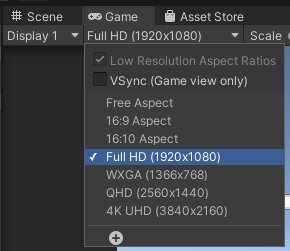
\includegraphics[width=0.3\linewidth]{rc/unity_set_ui_resolution_game}%
\hfill	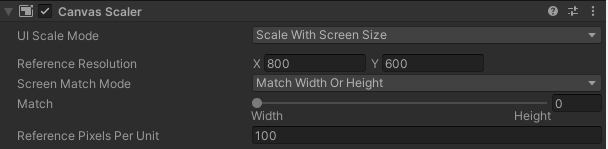
\includegraphics[width=0.6\linewidth]{rc/unity_set_ui_resolution_canvas_scaler}%
\hfill
\end{center}

Une fois cela réalisé, nous pouvons passer à la réalisation d'un widget complexe. Pour expliquer ce terme, nous allons réaliser un agglomérat de widgets existants avec un ou plusieurs scripts pour régir le comportement global du widget.

\section{Premier widget complexe: FormattedInputField}

L'objectif de ce widget est de réaliser une zone de texte qui change de couleur selon une expression régulière particulière comme sur l'image ci-dessous, où nous avons 3 \texttt{FormattedInputField}. Ainsi, lorsque la saisie est vide (le widget de gauche), nous avons une couleur standard. La présence d'un nombre engendre une couleur (le widget au centre) et une autre couleur si l'expression régulière n'est pas présente (le widget à droite).
\begin{center}
	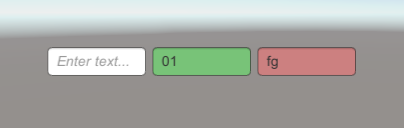
\includegraphics[width=0.4\linewidth]{rc/widget_formattetinputfield_start}
\end{center}

Pour cela, nous vous donnons le code suivant qui vient d'un programme \texttt{C\#} basique en dehors de \texttt{Unity}:

\begin{boxcode}
\begin{csharpsansbord}
Console.WriteLine("Regex experimentation");
string regex = "[0-9]+";
string montext = "bonjour";

if (System.Text.RegularExpressions.Regex.IsMatch(montext, regex))
	Console.WriteLine("Le texte matche la regex");
else
	Console.WriteLine("le texte ne matche pas la regex");

\end{csharpsansbord}
\end{boxcode}


D'un point de vue conceptuel, nous devons suivre les étapes suivantes (si vous faites autrement, tant pis pour vous, même si cela peut fonctionner):
\begin{enumerate}
	\item Créer les attributs publics correspondant aux couleurs et les initialiser directement.
	\item Créer l'attribut de la \texttt{regex} sous forme de chaîne de caractères.
	\item Réaliser la \texttt{callback} lorsqu'on change le texte dans le champ de saisie.
	\item La couleur qu'il faut changer est celle du composant image.
\end{enumerate}

\begin{info}
Pour réaliser le dernier point, il faut bien se rappeler de la séance précédente et de la partie sur l'\texttt{inspecteur} des objets en \texttt{Unity}. En effet, si on regarde bien, nous avons différents composants pour le champs de saisie. Le composant qui nous intéresse est l'\textbf{image} permettant de changer l'attribut \texttt{color} pour répondre à nos conditions. Pour cela, il nous suffit, à partir du \texttt{GameObject}, de récupérer l'objet souhaité:

\begin{csharp}
Image image = gameObject.GetComponent<Image>();
\end{csharp}

J'insiste que \texttt{GetComponent} récupère le premier composant du type souhaité dans le \texttt{GameObject} courant, il existe une version permettant de récupérer tous les composants d'un type cible.
\begin{csharp}
Image[] images = gameObject.GetComponents<Image>();
\end{csharp}
\end{info}

Réaliser le widget voulu, en attachant une importance à la hiérarchie dans la structure de votre projet et aux noms que vous adoptez (harmonisation et uniformisation).

\section{Widget: ComplexSlider}

Dans la section précédente, nous avions un unique widget. Ici, nous allons composer un widget complexe à partir de 3 widgets basiques. Pour cela, nous allons réaliser des curseurs complexes en composant un \texttt{texte} qui servira de label, d'un \texttt{slider} basique et d'un \texttt{champ de saisie} sur les nombres pour visualiser la valeur du \texttt{slider} et/ou la modifier manuellement. Ci-dessous, vous avez une image qui illustre deux \texttt{ComplexSlider} pour choisir des coordonnées \texttt{(x,y)}.

\begin{center}
	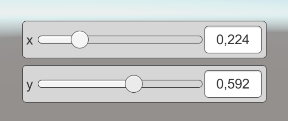
\includegraphics[width=0.5\linewidth]{rc/widget_complexslider_demo}
\end{center}

\begin{info}
Généralement un widget complexe doit avoir un panel à la base pour servir de fond visuel que vous opacifierez par défaut et qui permet de hiérarchiser les 3 sous-widgets le composant.
\end{info}

Vous devez réaliser un tel composant puis réaliser un unique script qui gouverne tous les aspects comportementaux. En particulier, lorsqu'une valeur est modifiée, cela impacte l'autre widget pour avoir toujours une cohérence entre le champ de saisie et le \texttt{slider} basique.

Pour cela, nous allons exploiter la hiérarchie de notre widget. Il existe deux mécaniques pour retrouver les enfants:
\begin{enumerate}
	\item \textit{via} les fonctions de recherche basées sur leur nom,
	\item \textit{via} les mécaniques de recherche sur un type souhaité.
\end{enumerate}
Réfléchissez sur les avantages et inconvénients des deux mécaniques en lisant la documentation associée à ces familles de fonctions: \url{https://docs.unity3d.com/ScriptReference/GameObject.html}.
En particulier, que se passe-t-il si plusieurs objets sont du même type? Ou si l'utilisateur modifie le nom d'un \texttt{sous-widget} ?.

\section{Exporter son travail}

Bravo, vous avez fait le plus gros. Demander à l'enseignant  qu'il vérifie votre développement ou critique vos noms et autres petits détails.

\subsection{Préfabriqué}
L'intéret de développer un widget est de pouvoir le réutiliser plusieurs fois sans devoir faire plusieurs manipulations identiques ou des \texttt{copier-coller}. Pour cela, \texttt{Unity} a la possibilité de créer des \texttt{Préfabs}, une sorte de sauvegarde de votre réalisation au sein d'un projet!

La procédure est assez simple: lorsque vous avez fini un \texttt{widget} qui n'a pas de dépendance extérieure, c'est-à-dire que le \texttt{widget} est autonome (sinon les dépendances risquent aussi d'être sauvegardées): il suffit de glisser le \texttt{GameObject} de la hiérarchie à la zone des \texttt{Assets}. Ainsi l'icône du \texttt{Gameobject} devient bleue! C'est ainsi qu'on sait qu'il s'agit d'un \texttt{Prefab}.


\begin{info}
Lorsque vous sélectionnez un \texttt{Prefab} dans la zone des \texttt{Assets}, vous avez un nouveau bouton dans l'\texttt{Inspecteur} qui vous permet de modifier ce \texttt{Prefab}.
\begin{center}
	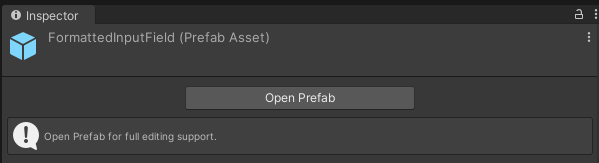
\includegraphics[width=0.5\linewidth]{rc/unity_set_ui_open_prefab}
\end{center}
\end{info}

\begin{attention}
Quand vous modifiez un \texttt{Prefab}, vous êtes dans un environnement particulier. Il est essentiel de revenir au plus vite dans le mode standard, en particulier pour sauvegarder et ainsi éviter des petits problèmes. 

Pour quitter, il faut cliquer sur le bouton "Retour" (noté par $'<'$) au niveau de la hiérarchie.
\begin{center}
	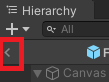
\includegraphics[width=0.3\linewidth]{rc/unity_set_ui_close_prefab}
\end{center}
\end{attention}

Réaliser des \texttt{Prefabs} de vos widgets en les ayant nettoyés si besoin AVANT! Ensuite, instancier pour expérimenter deux ou trois de vos \texttt{Prefabs}. Pour cela, il suffit de glisser votre \texttt{Prefab} depuis l'\texttt{Assert} vers la vue 3D ou la hiérarchie à l'endroit souhaité.

%\subsection{Export vers d'autres projets Unity}

\subsection{Export}

Maintenant que vous avez la possibilité de sauvegarder et réutiliser votre production au sein d'un projet, il est fréquent de devoir les exporter pour les utiliser dans d'autres projets. 
Pour cela, il faut exporter des \texttt{Prefabs} dont vous connaissez les dépendances, en sélectionnant votre \texttt{Prefab} dans les \texttt{Assets} et en faisant un clique droit dessus (attention, on vous demande de tester l'export d'un widget dans un premier temps, puis plusieurs widgets dans un second temps afin que vous compreniez les dépendances). Dans le menu contextuel, sélectionner \texttt{'Export Package\ldots'}.

Dans la nouvelle fenêtre, vous devez sélectionner les bonnes dépendances de votre widget. En particulier, \texttt{Unity} sélectionne par défaut tous les scripts sans distinction, car il n'arrive pas à calculer les dépendances correctement. Vous devez donc sélectionner les bonnes dépendances de scripts manuellement. Puis, cliquez sur le bouton \texttt{Export...} pour sauvegarder le package \texttt{Unity}.

\begin{center}
\hfill 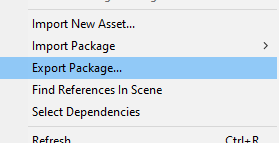
\includegraphics[width=0.35\linewidth]{rc/unity_set_ui_export_package}
\hfill 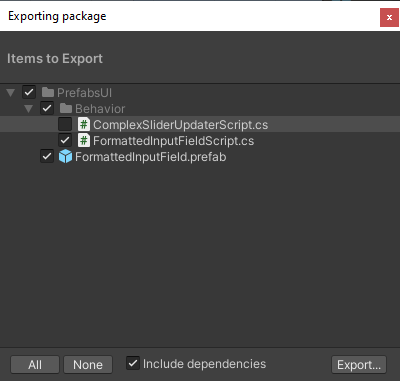
\includegraphics[width=0.5\linewidth]{rc/unity_set_ui_export_prefab_deps}
\hfill 
\end{center}

\subsection{Import}

Pour tester nos paquets \texttt{Unity} créés à l'étape précédente, c'est très simple! Il suffit de créer un nouveau projet \texttt{Unity} et glisser votre fichier \texttt{.unitypackage} dans les \texttt{Assets}, puis se laisser guider par le menu.

\begin{info}
Une alternative consiste  à faire juste un clique droit dans la zone des \texttt{Assets} et cliquer sur l'import d'un paquet personnalisé.
\end{info}

Votre widget est prêt à l'emploi. La mécanique des \texttt{Unity packages} est l'une des façons de se partager le travail lorsqu'on est plusieurs sur un même projet et que cela s'y prête bien. 

\section{Toujours plus loin}

\subsection{Des Prefabs partout !}
Reprendre votre TP précédent ou un nouveau projet qui exploite vos nouveaux widgets, histoire de voir une application complète et comprendre que votre \texttt{Prefab} doit bien être autonome pour embarquer uniquement son comportement intrinsèque!

\subsection{Retour sur la multi-résolution}
En reprenant l'hyperlien cité en introduction, vérifier que les \textit{ancres} des éléments du \texttt{Canvas} sont bien définies puis jouer avec le composant \texttt{Canvas Scaler} pour tester le positionnement de ces éléments. 

Tester également les résolutions proposées dans le \texttt{GameView}. Enfin, créer une résolution personnalisée (imiter un mode "Portrait" par exemple) et vérifier si les widgets sont toujours positionnés correctement.

\subsection{Orientation du Canvas}
À partir du lien \href{https://docs.unity3d.com/2022.3/Documentation/Manual/UICanvas.html}{UICanvas}, expérimenter les modes de rendu "\texttt{Screen Space - Camera}" et "\texttt{World Space}" pour modifier l'orientation et la position du \texttt{Canvas} et de ses enfants.
\end{document}
